\renewcommand{\BrainFuckChapter}{
  {-}{[}{-}{-}{-}{-}{-}{-}{-}{>}{+}{<}{]}{>}{-}{-}{-}{.}{[}{+}{+}{>}{-}{-}{-}{-}{-}{-}{-}{<}{]}{>}{.}{+}{+}{+}{+}{+}{.}{.}{-}{-}{[}{-}{>}{+}{+}{+}{<}{]}{>}{+}{.}{+}{+}{+}{+}{+}{.}{-}{-}{-}{-}{-}{-}{-}{-}{-}{.}{+}
  {+}{+}{+}{+}{+}{+}{.}{-}{>}{<}{-}{-}{<}{>}{<}{>}{<}{-}{-}{-}{+}{+}{+}{>}{-}{-}{<}{+}{>}{>}{<}{+}{>}{>}{<}{-}{<}{>}{+}{>}{<}{-}{+}{-}{+}{+}{>}{-}{+}{-}{-}{-}{>}{<}{<}{+}{+}{-}{+}{<}{>}{<}{<}{+}{<}{>}{+}{-}{+}{>}
}
\renewcommand{\LifeChapter}{y}

\chapter{\fuzzinel}
\label{sec:fuzzinel}
In this chapter we focus on addressing the \ac{SFL} limitations
explained in \CrefPageParen{sec:intro:research-goals:fuzzy-errors}.
%
Concretely, we propose a generalization to the \ac{SFL} diagnostic
framework, dubbed \fuzzinel{}\footnote{\fuzzinel{} is a combination of
  $50\%$ ``Fuzzy'' and $50\%$ ``Barinel'', which is the name of the
  original \ac{SFL} algorithm.}, capable of diagnosing fuzzy errors
with better accuracy.
%
This chapter is divided as follows.
%
First, we introduce our enhanced \ac{SFL} approach.
%
Second, we evaluate the performance of our approach.

\section{Approach}
\label{sec:fuzzinel:approach}
The problem of handling fuzzy errors can be divided in two
sub-problems: detection and diagnostic problems.
%
In this section we discuss how to solve both problems in the context
of \ac{SFL}.

\subsection{Fuzzy Error Detection}
\label{sec:fuzzinel:approach:fuzzy-error-detection}
Existent approaches to error detection (\eg,~\citep{Casanova13}) make
use of first-order logic descriptions of the correct behavior of the
system (weak-fault models) to assign transactions to one of two
possible sets: the pass set and the fail set ($P$ and $F$
respectively, where $F = \overline{P}$).
%
A consequence of such fault models is the \textit{crisp} distinction
between correct and incorrect system states.
%
While this classical logic description enables an accurate
representation of functional errors, it is unable to accurately
represent a large variety of non-functional errors.

As an example, consider a type of non-functional error that,
informally, is described by the statement ``The system is slow''.
%
Even though we can easily relate the slowness of the system to an
appropriate metric (\eg, response time), it is not easy to define a
crisp boundary in this same metric to distinguish acceptable and slow
transactions.
%
By setting a crisp boundary at, for instance, $1$ second, a response
time of $0.9999$ seconds would be considered to be correct whereas a
marginally superior response time would be considered incorrect.
%
Also, a response time of $0.9999$ seconds would result in the same
type of error information (pass) as a smaller response time even
though the larger response time may represent an error symptom.
%

To overcome the expressiveness limitation of the classical logic error
detection mechanisms, we propose their generalization using fuzzy
logic \citep{Zadeh65}.
%
Fuzzy logic extends the notion of binary set membership by introducing
the concept of membership functions, denoted $\fn{\mu_A}$ (membership
function for set $A$), mapping a set of problem-specific variables
onto the continuous interval $[0, 1]$, where the endpoints of $0$ and
$1$ conform to no membership and full membership, respectively.
%
In the context of error detection, the concept of fuzzy membership
enables the representation of $3$ types of system states: correct
($\ferror(x) = 0$), incorrect ($\ferror(x) = 1$) and degraded
($0 < \ferror(x) < 1$).
%
Intuitively, since $F = \overline{P}$, in the new fuzzy error model a
degraded transaction exhibits both correct and incorrect behaviors
simultaneously, however with different degrees.
%

\begin{figure}[!ht]
  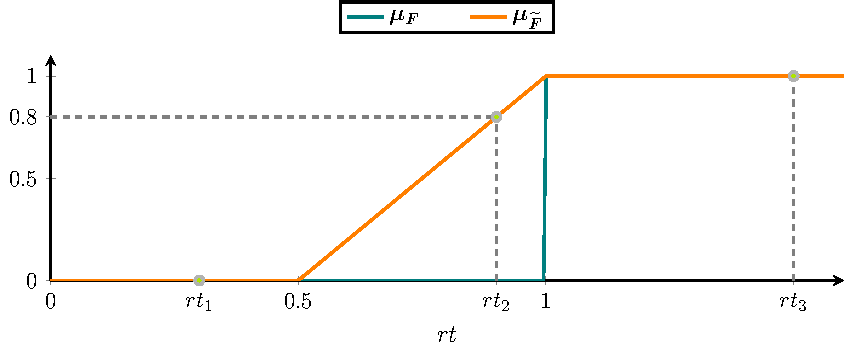
\includegraphics[page=1]{figures/fuzzinel/figures/main.pdf}
  \caption{Crisp \vs{} fuzzy sets\label{fig:fuzzinel:crisp-vs-fuzzy}}
\end{figure}


As an example, consider the crisp fail set containing all response
times ($rt$) above $1$ second.
%
This same set could be represented in terms of a membership function
as (\Cref{fig:fuzzinel:crisp-vs-fuzzy}):
\begin{equation}
  \cerror(rt) =
  \begin{cases}
    0 &,\ rt \leq 1 \\
    1 &,\ rt > 1
  \end{cases}
\end{equation}
%

To achieve the goal of representing the degraded state, consider that
all response times below $0.5$ seconds are considered correct and all
times above $1$ second incorrect.
%
Furthermore, consider that the amount of degradation follows a linear
pattern between those two thresholds.
%
The fuzzy fail set membership function representing this particular
type of error could be defined as:
\begin{equation}
  \label{eq:fuzzinel:fuzzy-error-fn}
  \ferror(rt) =
  \begin{cases}
    0       &,\ rt < 0.5 \\
    2 \cdot rt - 1 &,\ 0.5 \leq rt \leq 1 \\
    1       &,\ rt > 1
  \end{cases}
\end{equation}
%

\begin{figure}[!ht]
  \includegraphics[page=2]{figures/fuzzinel/figures/main.pdf}
  \caption{Arbitrary membership functions\label{fig:fuzzinel:arbitrary-error-fns}}
\end{figure}

It is important to note that the assumption of linear degradation
introduced in \Cref{eq:fuzzinel:fuzzy-error-fn} was only made for
simplicity.
%
In real-world scenarios, the membership functions are application
dependent and can exhibit arbitrary patterns.
%
From our approach's point-of-view, the membership functions are
treated as black-boxes.
%
\Cref{fig:fuzzinel:arbitrary-error-fns} shows a set of alternative
membership functions for the error previously described.
%
Despite their odd shapes they are acceptable membership functions,
provided that they correctly describe the error state of the
transaction.
%


\begin{figure}[!ht]
  \includegraphics[page=3]{figures/fuzzinel/figures/main.pdf}
  \caption{Error detection sensitivity intuition\label{fig:fuzzinel:sensitivity}}
\end{figure}

Furthermore, it is possible to change the error detection sensitivity
by raising $\ferror$ to an exponent, as depicted in \Cref{fig:fuzzinel:sensitivity}.
%
We can see that by raising $\ferror$ to an exponent in the
interval $]1,+\infty[$, the error detection becomes less sensitive to
errors in the fuzzy zone (\ie, the error value in the fuzzy zone
becomes smaller than the original).
%
In contrast, by raising $\ferror$ to an exponent in the
interval $]0,1[$, the error detection becomes more sensitive to errors
in the fuzzy zone.
%
In fact, when the exponent tends to either $+\infty$ or $0$, the fuzzy
membership becomes a binary membership and errors in the fuzzy zone
become passes and fails, respectively.

\begin{figure}[ht]
  \begin{tabular}{c|c|cc|cc}
    \multirow{2}{*}{$i$} & \multirow{2}{*}{$rt$} & \multicolumn{2}{c|}{$A$} & \multicolumn{2}{c}{$e$}                   \\\cline{3-6}
                         &                       & $c_1$                    & $c_2$ & $\cerror(rt_i)$ & $\ferror(rt_i)$ \\ \hline
    $1$                  & $0.3$                 & \nhit                    & \hit  & $0$             & $0$             \\
    $2$                  & $0.9$                 & \hit                     & \nhit & $0$             & $0.8$           \\
    $3$                  & $1.5$                 & \hit                     & \hit  & $1$             & $1$             \\
  \end{tabular}
  \caption{Fuzzy error hit spectrum example \label{fig:fuzzinel:spectrum-fuzzy-error}}
\end{figure}

To conclude the illustration of the fuzzy error detection process,
consider the spectrum presented in
\Cref{fig:fuzzinel:spectrum-fuzzy-error}, which also contains the
run-times for each transaction (marked in
\Cref{fig:fuzzinel:crisp-vs-fuzzy}).
%
From this spectrum we can see that, in particular for $t_2$, the crisp
error vector neglected an error symptom whereas the fuzzy error vector
categorized that same transaction as being $80\%$ degraded.



Finally, it is worth mentioning that, even though our simplistic
example only used one variable to determine the error value of the
transactions, the error value can be a function of an arbitrary number
of variables.
%
Furthermore, a system may have several membership function for
different types of transactions.

\subsection{Fuzzy Error Diagnosis}
\label{sec:fuzzinel:approach:fuzzy-error-diagnosis}
Using fuzzy logic to detect errors, it is possible to assert that a
particular transaction is $80\%$ degraded (\ie,
$\ferror=0.8$ and consequently $\ferror[P]=0.2$).
%
The remaining challenge consists in integrating this additional
knowledge in the diagnostic process.

As an example consider again the spectrum depicted in
\Cref{fig:fuzzinel:spectrum-fuzzy-error}.
%
Using the approach explained in \Cref{sec:intro:candidate-ranking}
(\ie, using $e = \cerror$), it follows that the
candidates%
%
\footnote{The candidates for the fuzzy approach are calculated by
  setting a threshold for $\ferror$ to discretize transactions in
  terms of pass/fail. In this example we use the threshold $\ferror =
  1$.}
%
$d_1 = \{c_1\}$ and $d_2= \{c_2\}$ are
ranked equally.
%
However, intuitively, we would expect $d_1$ to be ranked ahead of
$d_2$ since transaction $t_2$, in which component $c_1$ was involved,
shows error symptoms whereas $t_1$ does not.

To solve this limitation we make use of the concept of
probability of a fuzzy event \citep{Zadeh68}.
%
The probability of a fuzzy event is defined as:
\begin{equation}
  \pr{\alpha} = \sum_{x\in\Omega}{\fn{\mu_x}(\alpha) \cdot \pr{x}}
\end{equation}
\noindent where $\alpha$ is an arbitrary event, and $\Omega$ is a set
representing all the possible outcomes of $\alpha$.

Mapping this definition to the problem at hand, we generalize
\Cref{eq:intro:likelihood-func} as:
\begin{equation}
  \label{eq:fuzzinel:likelihood-generalization}
  \begin{split} \likelihoodi{} &= \underbrace{e_i \cdot \big(1 -
      \gFunc{}\big)}_{x = F} \\
    &+ \underbrace{\vphantom{\big(}(1-e_i) \cdot \gFunc{}}_{x = P}
  \end{split}
\end{equation}
\noindent
where the first part of the equation ($x=F$) accounts for the
incorrect behavior whereas the second part ($x=P$) accounts for the
correct behavior.
%
In contrast to \Cref{eq:intro:likelihood-func}, this generalization is valid for
fuzzy error values (\ie, $e \in ]0,1[$).
%
\Cref{fig:fuzzinel:likelihood-generalization} shows the plot of the
\Cref{eq:fuzzinel:likelihood-generalization} with respect to $e_i$ and
$\gFunc{}$.
%
For comparison, we also plot \Cref{eq:intro:likelihood-func} with thick
black lines.
\begin{figure}[ht]
  \includegraphics[page=4]{figures/fuzzinel/figures/main.pdf}
  \\
  \begin{subfigure}{0.48\columnwidth}
    \includegraphics[page=5]{figures/fuzzinel/figures/main.pdf}
    \caption{2D view}
  \end{subfigure}
  \hfill{}
  \begin{subfigure}{0.48\columnwidth}
    \includegraphics[page=6]{figures/fuzzinel/figures/main.pdf}
    \caption{3D view}
  \end{subfigure}
  \caption{Likelihood function plot\label{fig:fuzzinel:likelihood-generalization}}
\end{figure}



Using the above generalization, the probabilities of the two
candidates are calculated as follows:
\begin{equation}
  \begin{split} \likelihood[d_1]{} &= \underbrace{(0.8 \cdot (1-g_1) +
      (1 - 0.8) \cdot g_1)}_{t_2} \\ &\times \underbrace{(1 \cdot (1-g_1) +
      (1 - 1) \cdot g_1)}_{t_3}\\
    &= \underbrace{(0.8 \cdot (1 - g_1) + 0.2 \cdot g_1)}_{t_2} \times \underbrace{(1 - g_1)}_{t_3}
  \end{split}
\end{equation}

\penalty-10000
\begin{equation}
  \begin{split}
    \likelihood[d_2]{} &= \underbrace{(0 \cdot (1-g_2) + (1- 0) \cdot g_2)}_{t_1} \\
    &\times \underbrace{(1 \cdot (1-g_2) + (1 - 1) \cdot g_2)}_{t_3}\\
    &= \underbrace{\vphantom{(}g_2}_{t_1} \times \underbrace{(1 - g_2)}_{t_3}
  \end{split}
\end{equation}

\begin{figure}[!ht]
  \begin{subfigure}{0.45\columnwidth}
    \includegraphics[page=7]{figures/fuzzinel/figures/main.pdf}
    \caption{$\likelihood[d_1]$}
  \end{subfigure}
  %
  \begin{subfigure}{0.45\columnwidth}
    \includegraphics[page=8]{figures/fuzzinel/figures/main.pdf}
    \caption{$\likelihood[d_2]$}
  \end{subfigure}

  \caption{Likelihood plots \label{fig:fuzzinel:likelihood-plots}}
\end{figure}


By performing an \ac{MLE} for both functions
(\Cref{fig:fuzzinel:likelihood-plots}) it follows that
$\likelihood[d_1]{}$ is maximized for $g_1=0$ and $\likelihood[d_2]{}$
for $g_2 = 0.5$.
%
Applying the maximizing values to both expressions, it follows that
$\posterior[d_1]{} \approx 8\e{-4}$ and $\posterior[d_2]{} \approx 2.5\e{-4}$.
%
Such probabilities entail the ranking $\angledlist{d_1, d_2}$,
which breaks the ambiguity between $d_1$ and $d_2$, thus improving the
diagnostic accuracy.

\section{Benchmark}
\label{sec:fuzzinel:benchmark}
In this section we describe our benchmark approach and discuss
results.
%


\subsection{Setup}
To evaluate our approach we make use of a simulator as proposed in
\citep{Chen13}\footnote{\url{https://github.com/SERG-Delft/sfl-simulator}}.
%
The simulator provides functions to describe and execute a
probabilistic model of an arbitrary system, thereby gathering the
required spectra.
%
The authors showed that, in the scope of \ac{SFL}, the benchmark
results for both real and synthetic data are comparable.
%
This is mainly due to the fact that, since system is highly
abstracted, the spectra generated by real and simulated systems is
similar.
%


\begin{figure}[!ht]
  \includegraphics[page=9]{figures/fuzzinel/figures/main.pdf}
  \caption{Probabilistic topology model\label{fig:fuzzinel:probabilistic-model}}
\end{figure}


Our simulator consists of a stack automaton which takes as input a
probabilistic model of the system (such as, for instance, the one
depicted in \Cref{fig:fuzzinel:probabilistic-model}) and, through a
Monte Carlo process, generates spectra.
%
The probabilistic model describes the system's topology, the
interaction between components, and the system's faults.
%
To build the topology portion of the model, two primitives exist:
components and links (depicted in blue and orange colors, respectively).
%
Concretely, a component (identified by its numeric ID) contains a list
of links.
%
A link consists of a list of component IDs with associated transition
probabilities ($\emptyset$ corresponds to no transition).

Whenever a component is activated, its links are sequentially
evaluated.
%
The evaluation of a link consists of pushing the component's next link
onto the stack (if it exists) and randomly selecting a component
(based on the transition probabilities defined in the activated link)
to continue the execution.
% $
When all the links belonging to a component have been evaluated, a
link is popped from the call stack, returning the control to the
caller component.
%
As soon as all the links belonging to a component have been evaluated
and the stack is empty, the execution halts.

Considering the description of the simulator, a transaction can be
generated by pushing the first link of a component marked as an entry
point onto the stack ($c_0$ in
\Cref{fig:fuzzinel:probabilistic-model}) and running the simulator
from that state until its execution comes to a stop.
%
The spectrum is generated by repeating this process an arbitrary
number of times while recording which components have been activated
in each transaction.

To emulate the error behavior, components may be injected with faults
(depicted in red), which are parameterized over $4$ variables ($p_c$,
$p_d$, $p_i$, and $p_f$).
%
$p_c$, $p_d$, and $p_i$ correspond to the probabilities of correct,
degraded, and incorrect behavior.
%
During the simulation, whenever a faulty component is activated, the
outcome of such activation (in terms of correct, degraded, or
incorrect) is randomly determined using such probabilities.
%
In the event of a component performing erroneously, it has an
associated probability $p_f$ of failure which, whenever it occurs, it
results in an premature end of the transaction (in
\Cref{fig:fuzzinel:probabilistic-model}, an error in component $c_4$
always results in a failure whereas an error in component $c_1$ only
has a $40\%$ chance of resulting in a failure).
%
To determine the transaction's fuzzy error value, we apply the
following rules:
\begin{equation}
  e = \begin{cases}
    1, & \text{if at least one component performed
      erroneously} \\
    0, & \text{if all components performed
      correctly} \\
    \fn{rand}(0,1), & \text{otherwise\footnote{This
        happens if no component performed erroneously, but at least one
        faulty component exhibited a degraded performance.}}
  \end{cases}
\end{equation}




To generate the spectra required for our benchmark we undergo
a two-step process.
%
In the first stage we randomly generate a set of system models, while
in the second, we use such models to generate the required spectra.

\begin{figure}[ht]
  \includegraphics[page=10]{figures/fuzzinel/figures/main.pdf}
  \caption{N-tier service architecture\label{fig:fuzzinel:ntier}}
\end{figure}

We generated system models that comply with a N-tier service
architecture (\Cref{fig:fuzzinel:ntier}).
%
Systems were created by randomly selecting the number of tiers ($T \in
[3,10]$) as well as the number of components in each tier ($C_i \in
[3,10], 1 \leq i \leq T$).
%
Every component is connected to all the components of the next tier
with random transition probabilities.
%
To exhibit erroneous behavior, a number of faults ($F$) was randomly
injected (in terms of position) in the systems.

In our setup, we generated $100$ systems for each value $F \in [2,4]$,
totaling $300$ systems.
%
The injected faults had $90\%$ and $10\%$ probabilities of degraded,
and erroneous behavior, respectively.
%

The spectra generation is parameterized over a single variable $E$,
representing the number of errors at the end of which the simulation
stops.
%
For each generated system, we ran $10$ simulations for each value $E
\in [1,9]$, totaling $90$ spectra per system.
%
Overall, our benchmark is composed of $300 \times 90 = 27000$ test
cases.


\subsection{Evaluation Metric}
The wasted effort metric evaluates, for a particular diagnostic
report, how many healthy components need to be inspected before all
faulty components are found \citep{Steimann13}.
%
To calculate this metric one must undergo an iterative process.
%
Starting with the first candidate, all the candidate's components are
inspected to determine whether that particular component was
responsible for the erroneous behavior.
%
Depending on the result of such inspection two outcomes may occur.
%
On the one hand, if the component is found to be faulty, that particular
component is removed from all other candidates in the ranking.
%
On the other hand, if the component is found to be healthy, all
candidates in the ranking containing that particular component are
removed.
%
This process is repeated until all faulty components are found.
%
In the case of the last inspected candidate being tied with other
candidates, it is assumed that, on average, half of the healthy
components are examined.

During this iterative process, we keep track of two counters:
inspected components ($I$) and faulty components ($C$).
%
Using these two counters, the wasted effort metric is calculated as
\begin{equation}
  W = I - C
\end{equation}

\begin{figure}[ht]
  \begin{tabular}[m]{c|c|c||c|c}
    & $d$   &  Rank & $I$ & $C$\\\hline
    $1$ & $\{c_1,c_4\}$            & $1$ & $2$ & $1$\\
    $2$ & \sout{$\{c_2,c_3,c_4\}$} & $2$ &  & \\
    $3$ & \sout{$\{c_3,c_4,c_5\}$} & $3$ &  & \\
    $4$ & $\{$\sout{$c_1$}$,c_2\}$ & $4$ &\multirow{2}{*}{$4$} & \multirow{2}{*}{$2$}\\
    $5$ & $\{c_3,c_5\}$            & $4$ &   & \\
  \end{tabular}
  \caption{Example diagnostic report\label{fig:fuzzinel:candidate-ranking}}
\end{figure}

As an example consider the diagnostic report presented in
\Cref{fig:fuzzinel:candidate-ranking} for which the correct
diagnostic candidate is $d = \{c_1,c_2\}$.
%
In order to calculate the wasted effort, we start by examining $c_1$
and $c_4$ finding that $c_1$ is faulty while $c_4$ is healthy.
%
Due to $c_4$ being healthy, candidates $d_2$ and $d_3$ are discarded.
%
Examining $d_4$ we observe that the only unexplored component ($c_2$) is faulty.
%
Additionally, we see that both system's faults were discovered.
%
However, as $d_5$ is tied with $d_4$, we must inspect half of the
healthy components.
%
The wasted effort of this diagnosis is therefore $W = 4 - 2 = 2$,
meaning that $2$ healthy components ($c_4$ and $c_3/c_5$) were
examined in the process of finding the root cause of the system's
errors.

A normalized version of the wasted effort is called \emph{diagnostic
  quality} and is defined as:
\begin{equation}
  Q = 1 - \frac{W}{M - C}
\end{equation}
\noindent
where $M$ is the number of system components.
%
The diagnostic quality value is between zero and one and estimates the
fraction of system's healthy components that need to be examined
before all faulty components are found.



We refine the diagnostic quality metric to take into account the fact
that, for a specific spectrum, not all components of the systems can be
at fault.
%
As an example consider a system with $1000$ components with a spectrum
consisting of a single failing transaction activating $2$ components.
%
Assuming the diagnostic algorithm only proposes plausible\footnote{By
  plausible we mean that all the candidate's components were at least
  activated once in an erroneous transaction.} candidates, the quality is
contained in the interval between $1$ and $\frac{999}{1000}$.
%
Instead of calculating the diagnostic quality using the $M$ components
of the system, we use $M_s$, the number of ``suspicious'' components
to calculate the new metric, which shall be referred to as ``fair
quality'' ($Q_f$).
%
A component is said to be suspicious if it was activated in a failing
transaction.
%
A consequence of using $Q_f$ is that the diagnostic qualities of all
possible permutations of the ranking always have a lower bound quality of 0.




\subsection{Results}
\label{sec:fuzzinel:benchmark:results}
In this section, we compare the performance of the crisp diagnostic
approach (\CrefPageSee{sec:intro:candidate-ranking}) with our fuzzy
approach for the generated spectra.
%
\begin{figure}[ht]
  \begin{center}
    \begin{subfigure}{0.43\columnwidth}
      \setlength{\fboxsep}{0em}
      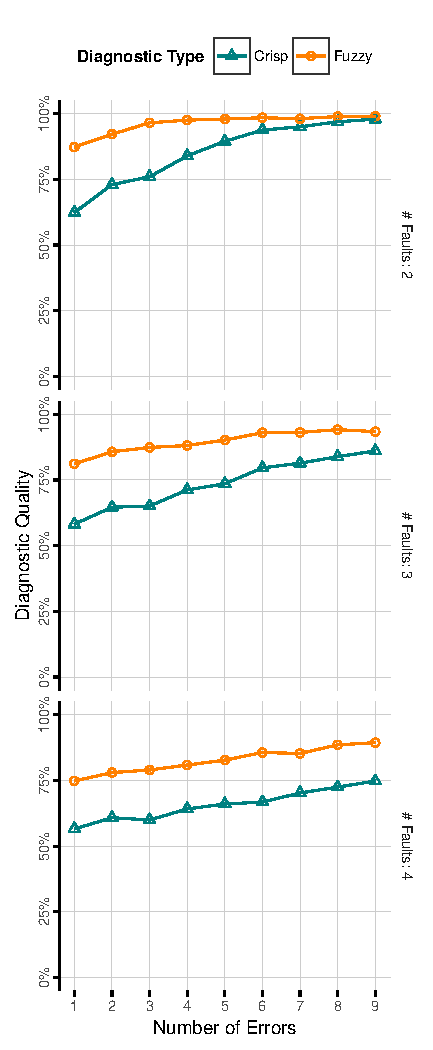
\includegraphics[trim=0.6em 0.5em 2.2em 1em,clip=true]{figures/fuzzinel/figures/plot2.pdf}
      \caption{Averages\label{fig:fuzzinel:res1}}
    \end{subfigure}%
    \begin{subfigure}{0.57\columnwidth}
      \setlength{\fboxsep}{0em}
      \noindent
      \includegraphics[trim=3em 0.5em 0.5em 1em,clip=true]{figures/fuzzinel/figures/plot3.pdf}
      \caption{Box plots\label{fig:fuzzinel:res3}}
    \end{subfigure}
  \end{center}
  \caption{Benchmark results}
\end{figure}

In \Cref{fig:fuzzinel:res1}, we compare the average $Q_f$ for each test scenario.
%
From the analysis of the plot we can see that the crisp approach was,
on average, outperformed by the fuzzy approach.
%
This is due to the fact that the fuzzy approach is able to
successfully take advantage of the extra fuzzy error information to
break the ties in the ranking (as shown in the example from
\Cref{fig:fuzzinel:spectrum-fuzzy-error}) that occur when dealing with
small numbers of erroneous transactions.
%
Furthermore, with the increase of erroneous transactions, it appears
that the average crisp approach's $Q_f$ seems to converge towards to
the same average $Q_f$ as the fuzzy approach.
%
This happens due to the fact that the information introduced by the
occurrence of errors eventually compensates for the limitations
imposed by the crisp error abstraction.
%

In \Cref{fig:fuzzinel:res3}, we present a set of box plots\footnote{For
  each test scenario, the box corresponds to $2^{nd}$ and $3^{rd}$
  quartiles (\ie, $50\%$ of the cases), the vertical lines correspond
  to the $1^{st}$ and $4^{th}$ quartiles, and the small dashes
  correspond to test cases categorized as outliers. A test case is
  considered to be an outlier if its distance from the box is greater
  that $1.5 * IQR$ (inter-quartile range, \ie, the height of the
  box).}  comparing the diagnostic quality distributions of both
approaches for each test scenario.
%
From the analysis of the plots we can see that the fuzzy approach not
only has a better performance than the crisp approach, but also that
the fuzzy approach distribution is more skewed towards better quality
results than the crisp approach.
%
Additionally, we can see that the fuzzy approach exhibits a higher
consistency (\ie, smaller inter-quartile range) than the crisp
approach.
%
This tendency can be further observed in \Cref{fig:fuzzinel:res4},
where we plot a more detailed version of \Cref{fig:fuzzinel:res3}, in
which we include every test case result.\footnote{To improve the
  visualization, we added transparency and random horizontal
  displacement to each data point.}
%


\begin{figure}[!ht]
  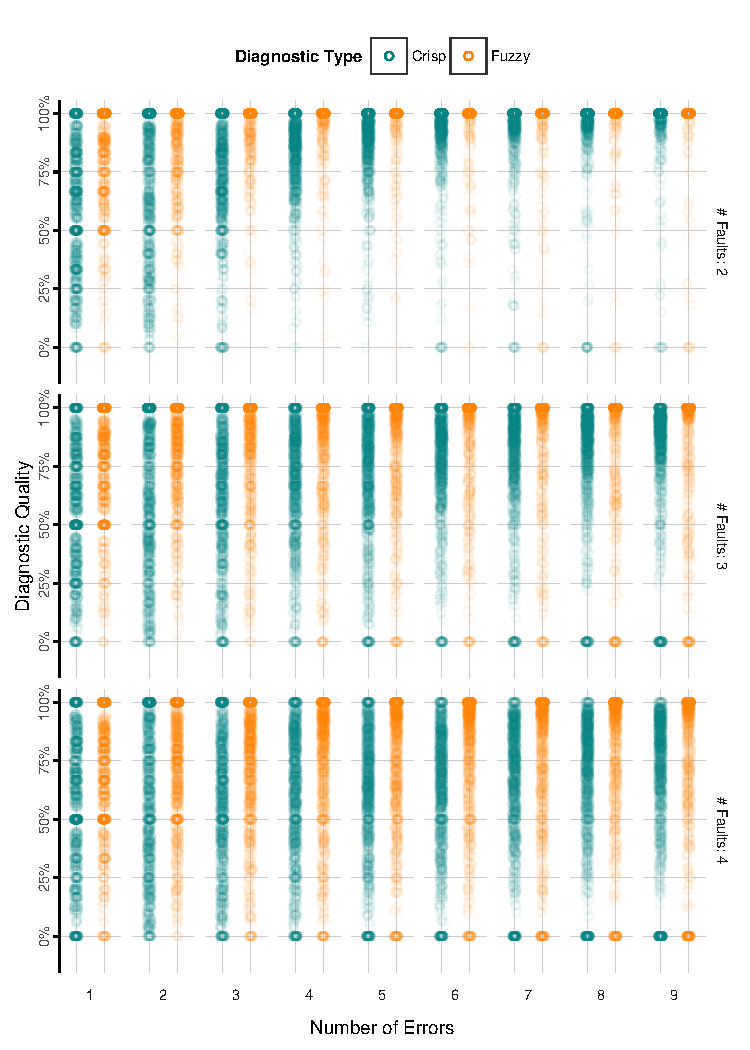
\includegraphics[width=\columnwidth]{figures/fuzzinel/figures/plot4.pdf}
  \caption{Benchmark results (detailed view)
    \label{fig:fuzzinel:res4}}
\end{figure}
\FloatBarrier


A pairwise analysis of the data (\Cref{fig:fuzzinel:res2}) shows that
our approach outperformed the crisp approach in $65\%$ of the test
cases.
%
Moreover, in $94\%$ of the cases our approach was at least as accurate
as the classical approach.
%
In the remaining $6\%$ of the test cases the accuracy loss was due to
\begin{inparaenum}[(1)]
\item lack of observations, and
\item marginal variations in the posterior probability but large
  enough to make the relative ranking change.
\end{inparaenum}
%
The overall average improvement of quality introduced by our algorithm
was of $\Delta Q_f = 0.153$, representing a relative improvement of $21\%$.
%
By performing a paired one-tailed T-test, we can ascertain that our
approach introduced a relative improvement of $20\%$, with a $99\%$
confidence interval.

\begin{figure}[!ht]
  \begin{tikzpicture}
    \tikzstyle{filled}=[inner sep=1mm,fill=white!100!black,draw, rounded corners=0.5mm,thick, align=center];

    \begin{pgfonlayer}{background}
      \node[anchor=south] (main) at (0,0){
        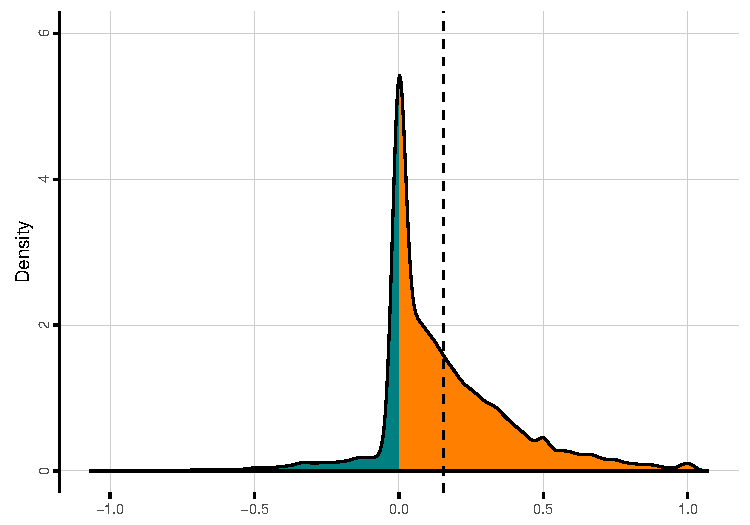
\includegraphics[trim=0em 0.5em 0cm 0cm,clip=true]
        {figures/fuzzinel/figures/plot1}};
    \end{pgfonlayer}
    \node[anchor=north,below=0cm of main.south] {$Q_f(${\color{dkclrb}Fuzzy}$) - Q_f(${\color{dkclra}Crisp}$)$};

    \node[filled,anchor=center] (eq) at (0.3,3) {$29\%$};
    \node[filled,anchor=east,right=2cm of eq.west] {$65\%$};
    \node[filled,anchor=west,left=2cm of eq.east] {$6\%$};

    \node[filled,anchor=west] at (0.6,7)  (f3) {
      $Q_f(${\color{dkclrb}Fuzzy}$) \geq
      Q_f(${\color{dkclra}Crisp}$)$: $94\%$ \\[0.5em]
      Relative $Q_f$ Improvement: $21\%$};

  \end{tikzpicture}
  \vspace{0.5em}
  \caption{Quality improvement density plot\label{fig:fuzzinel:res2}}
\end{figure}


\section{Summary}
In this chapter we successfully addressed the limitations presented in
\CrefPageParen{sec:intro:research-goals:fuzzy-errors} thereby
answering
\Cref{rq:fuzzy-error-encoding,rq:SFL-fuzzy-error-generalization}
(\pagerefTwo[, respectively] {rq:fuzzy-error-encoding}
{rq:SFL-fuzzy-error-generalization}).
%
Concretely, in this chapter:

\begin{itemize}[nolistsep]
\item We addressed \Cref{rq:fuzzy-error-encoding} by using fuzzy
  logic instead of the classical binary logic to detect/encode error
  states (\CrefPageSee[]{sec:fuzzinel:approach:fuzzy-error-detection}).
\item We addressed \Cref{rq:SFL-fuzzy-error-generalization} by
  generalizing the state-of-the-art \ac{SFL} using the concept of
  probability of a fuzzy event
  (\CrefPageSee[]{sec:fuzzinel:approach:fuzzy-error-diagnosis}).
\item We presented the conducted benchmarks showing that our fuzzy
  error approach (\CrefPageSee[]{sec:fuzzinel:benchmark:results}):
  \begin{itemize}
  \item Improved the diagnostic quality in $65\%$ of the test cases.
  \item Performed at least as good as the classical approach in $94\%$
    of the test cases.
  \item The average relative improvement introduced by our approach
    was of $20\%$, with a $99\%$ confidence interval.
  \end{itemize}
\end{itemize}
